\documentclass[10pt,a4paper]{article}
\usepackage[utf8]{inputenc}
\usepackage[brazilian]{babel}
\usepackage{lmodern}
\usepackage[left=2.5cm, right=2.5cm, top=2.5cm, bottom=2.5cm]{geometry}

\usepackage[mm]{zeuscolor}
\usepackage{zeusproblems}
\usepackage{zeustitle}
\usepackage{multicol}

\title{Martingales}
\author{Guilherme Zeus Moura}
\mail{zeusdanmou@gmail.com}
\titlel{Turma Olímpica}
\titler{\today}

\renewcommand\playerA[1]{Guilherme}
\renewcommand\playerB[1]{Zeus}

\begin{document}	
	\zeustitle
	\begin{exmp}
		Imagine os seguintes dados:
		\begin{itemize}
			\item O dado $A$ tem lados $2$, $2$, $4$, $4$, $9$, $9$.
			\item O dado $B$ tem lados $1$, $1$, $6$, $6$, $8$, $8$.
			\item O dado $C$ tem lados $3$, $3$, $5$, $5$, $7$, $7$.	
		\end{itemize}

		Se jogarmos os dados $A$ e $B$, a chance do número que sair no dado $A$ ser maior que o número que sair no $B$ é $\frac{5}{9}$.

		Se jogarmos os dados $B$ e $C$, a chance do número que sair no dado $B$ ser maior que o número que sair no $C$ é $\frac{5}{9}$.

		Se jogarmos os dados $A$ e $C$, qual é a chance do número que sair no dado $A$ ser maior que o número que sair no $C$?
	\end{exmp}

	\begin{exmp}[Dados de Grime]
		Outros dados legais:
	
		\begin{multicols}{2}
		
			\begin{tabular}{rl}
			Vermelho: & 4, 4, 4, 4, 4, 9\\
			Amarelo:  & 3, 3, 3, 3, 8, 8\\
			Azul:     & 2, 2, 2, 7, 7, 7\\
			Magenta:  & 1, 1, 6, 6, 6, 6\\
			Verde:    & 0, 5, 5, 5, 5, 5
		\end{tabular}
	
	
	\begin{center}
		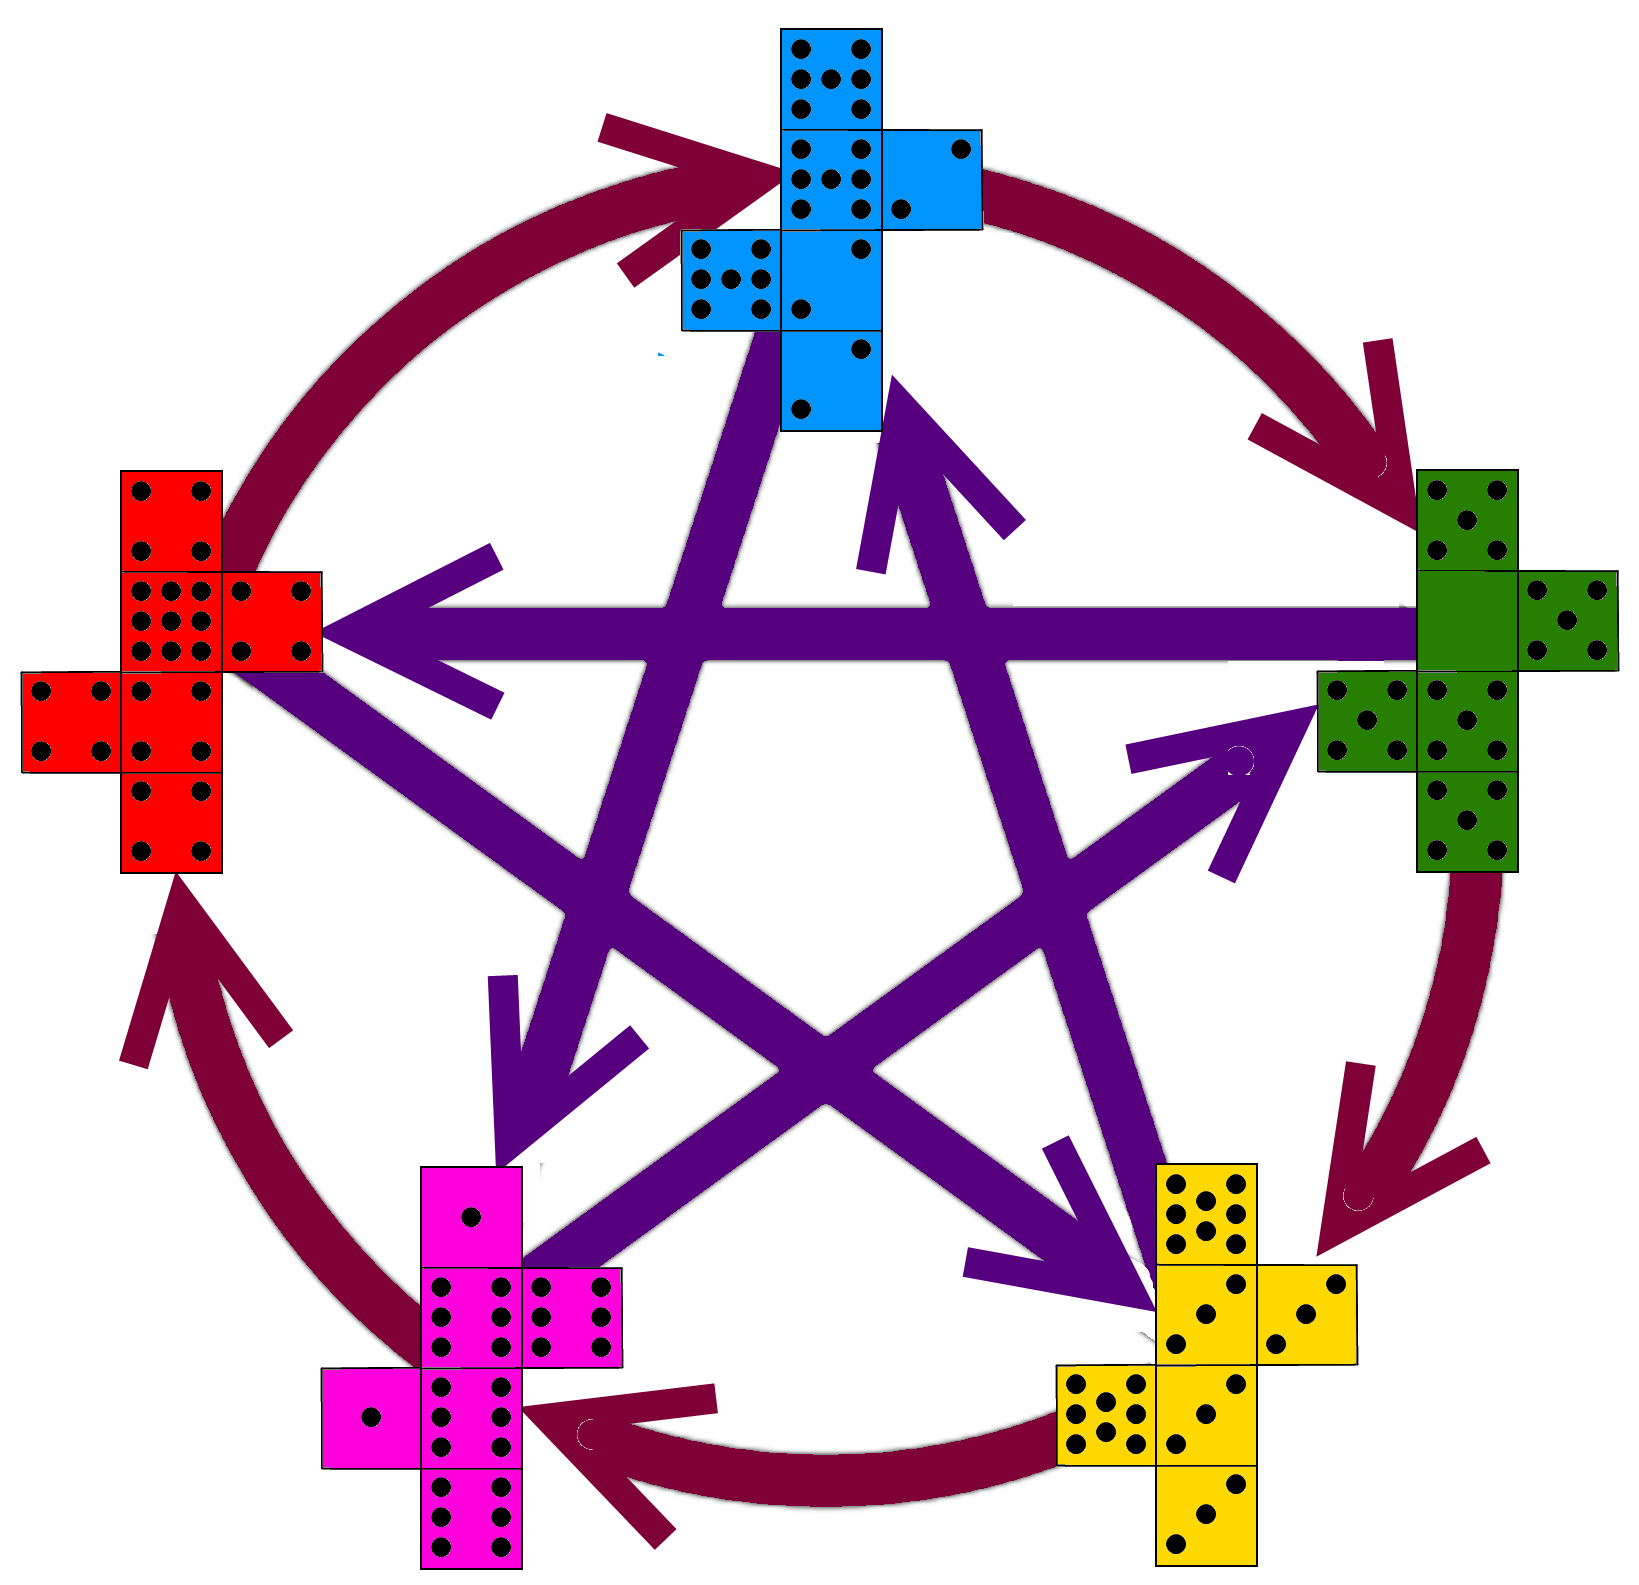
\includegraphics[width=0.2\textwidth]{diagram1.png}
	\end{center}

	\end{multicols}

	\end{exmp}

	\begin{exmp}[Jogo de Penney]
		O jogo involve jogar uma moeda, com igual probabilidade de cair cara $(H)$ ou coroa $(T)$. O jogo é jogado por dois jogadores, \playerA{$A$} e \playerB{$B$}, que escolhem sequências de três resultados. Por exemplo, suponha que \playerA{o jogador $A$} escolheu $HHH$ e \playerB{o jogador $B$} escolheu $THH$. Quando a moeda é jogada repetidamente, a sequência é algo do tipo:
		
		$$HTHTHHHHTHHHTTTTHTHH\dots$$

		O jogador cuja sequência aparecer primeiro ($HHH$ para \playerA{o jogador $A$} ou $THH$ para \playerB{o jogador $B$}) é declarado o vencedor.
	\end{exmp}

	\begin{defn}
		Um jogo justo (de tempo discreto) é uma sequência de variáveis aleatórias $X_1, X_2, \dots$ que satisfaz, para qualquer tempo $n$:
		\begin{gather*}
			\EE(|X_n|) < \infty;\\
			\EE(X_{n+1} \mid X_n, \dots, X_1) = X_n.
		\end{gather*}
	\end{defn}

	\begin{cor}
	Para os nossos propósitos, um jogo \emph{justo} é um jogo em que o $\EE(\Delta\text{dinheiro}) = 0$.
	\end{cor}

	\begin{thm}[Teorema Fundamental das Apostas / Optional Stopping Theorem]
		Seja $J$ um jogo justo. Qualquer estratégia de iterar $J$ que:
		\begin{itemize}
			\item termina quase certamente (isto é, $\PP = 1$) em tempo limitado por uma constante;
			\item termina com dinheiro limitado
		\end{itemize}
		é justa.
	\end{thm}

	\prob{Um sorteador de letras a cada minuto, sorteia uma letra \texttt{A-Z}. Qual o tempo médio até aparecer a palavra \texttt{ABRACADABRA}?}	

	\begin{sol}
		Vamos inventar alguns jogos:

		$J(X):$ aposta $N$ moedas para jogar. Ganha $26N$ moedas, se cair a letra $X$.

		$J^*:$ Aposta $1$ moeda para jogar. Aposta $1$ jogando em $J(\mathtt{A})$. Se ganhar, aposta tudo em $J(\mathtt{B})$. Se ganhar, aposta tudo em $J(\mathtt{R})$. E assim por diante. Se perder em algum momento, sai do jogo.

		$J$ é justo, pois o valor esperado de dinheiro é 0. $J^*$ é um jogo justo, pois é uma iteração de $J$ e termina com dinheiro limitado.

		Vamos jogar diversos jogos $J^*$ simultâneamente, começando a jogar um novo jogo $J^*$ a cada minuto e vamos parar imediatamente de jogar todos os jogos quando ganharmos o prêmio final em algum dos jogos $J$

		Como é justo, o dinheiro esperado é $0$. Quando finalmente ganharmos o jogo, três de nossos jogos estarão rodando são: \texttt{ABRACADABRA} \texttt{ABRA} e \texttt{A}.

		Portanto, ganharemos $26^{11} + 26^4 + 26$ no fim do jogo. Porém, perdemos $T$ moedas, onde $T$ é o número de minutos que passaram. Como o dinheiro esperado é $0 = 26^{11} + 26^4 + 26 - T$, temos que $T = 26^{11} + 26^4 + 26$.
	\end{sol}
\end{document}
